% Options for packages loaded elsewhere
\PassOptionsToPackage{unicode}{hyperref}
\PassOptionsToPackage{hyphens}{url}
\PassOptionsToPackage{dvipsnames,svgnames,x11names}{xcolor}
%
\documentclass[
  letterpaper,
  DIV=11,
  numbers=noendperiod]{scrreprt}

\usepackage{amsmath,amssymb}
\usepackage{iftex}
\ifPDFTeX
  \usepackage[T1]{fontenc}
  \usepackage[utf8]{inputenc}
  \usepackage{textcomp} % provide euro and other symbols
\else % if luatex or xetex
  \usepackage{unicode-math}
  \defaultfontfeatures{Scale=MatchLowercase}
  \defaultfontfeatures[\rmfamily]{Ligatures=TeX,Scale=1}
\fi
\usepackage{lmodern}
\ifPDFTeX\else  
    % xetex/luatex font selection
\fi
% Use upquote if available, for straight quotes in verbatim environments
\IfFileExists{upquote.sty}{\usepackage{upquote}}{}
\IfFileExists{microtype.sty}{% use microtype if available
  \usepackage[]{microtype}
  \UseMicrotypeSet[protrusion]{basicmath} % disable protrusion for tt fonts
}{}
\makeatletter
\@ifundefined{KOMAClassName}{% if non-KOMA class
  \IfFileExists{parskip.sty}{%
    \usepackage{parskip}
  }{% else
    \setlength{\parindent}{0pt}
    \setlength{\parskip}{6pt plus 2pt minus 1pt}}
}{% if KOMA class
  \KOMAoptions{parskip=half}}
\makeatother
\usepackage{xcolor}
\setlength{\emergencystretch}{3em} % prevent overfull lines
\setcounter{secnumdepth}{5}
% Make \paragraph and \subparagraph free-standing
\makeatletter
\ifx\paragraph\undefined\else
  \let\oldparagraph\paragraph
  \renewcommand{\paragraph}{
    \@ifstar
      \xxxParagraphStar
      \xxxParagraphNoStar
  }
  \newcommand{\xxxParagraphStar}[1]{\oldparagraph*{#1}\mbox{}}
  \newcommand{\xxxParagraphNoStar}[1]{\oldparagraph{#1}\mbox{}}
\fi
\ifx\subparagraph\undefined\else
  \let\oldsubparagraph\subparagraph
  \renewcommand{\subparagraph}{
    \@ifstar
      \xxxSubParagraphStar
      \xxxSubParagraphNoStar
  }
  \newcommand{\xxxSubParagraphStar}[1]{\oldsubparagraph*{#1}\mbox{}}
  \newcommand{\xxxSubParagraphNoStar}[1]{\oldsubparagraph{#1}\mbox{}}
\fi
\makeatother

\usepackage{color}
\usepackage{fancyvrb}
\newcommand{\VerbBar}{|}
\newcommand{\VERB}{\Verb[commandchars=\\\{\}]}
\DefineVerbatimEnvironment{Highlighting}{Verbatim}{commandchars=\\\{\}}
% Add ',fontsize=\small' for more characters per line
\usepackage{framed}
\definecolor{shadecolor}{RGB}{241,243,245}
\newenvironment{Shaded}{\begin{snugshade}}{\end{snugshade}}
\newcommand{\AlertTok}[1]{\textcolor[rgb]{0.68,0.00,0.00}{#1}}
\newcommand{\AnnotationTok}[1]{\textcolor[rgb]{0.37,0.37,0.37}{#1}}
\newcommand{\AttributeTok}[1]{\textcolor[rgb]{0.40,0.45,0.13}{#1}}
\newcommand{\BaseNTok}[1]{\textcolor[rgb]{0.68,0.00,0.00}{#1}}
\newcommand{\BuiltInTok}[1]{\textcolor[rgb]{0.00,0.23,0.31}{#1}}
\newcommand{\CharTok}[1]{\textcolor[rgb]{0.13,0.47,0.30}{#1}}
\newcommand{\CommentTok}[1]{\textcolor[rgb]{0.37,0.37,0.37}{#1}}
\newcommand{\CommentVarTok}[1]{\textcolor[rgb]{0.37,0.37,0.37}{\textit{#1}}}
\newcommand{\ConstantTok}[1]{\textcolor[rgb]{0.56,0.35,0.01}{#1}}
\newcommand{\ControlFlowTok}[1]{\textcolor[rgb]{0.00,0.23,0.31}{\textbf{#1}}}
\newcommand{\DataTypeTok}[1]{\textcolor[rgb]{0.68,0.00,0.00}{#1}}
\newcommand{\DecValTok}[1]{\textcolor[rgb]{0.68,0.00,0.00}{#1}}
\newcommand{\DocumentationTok}[1]{\textcolor[rgb]{0.37,0.37,0.37}{\textit{#1}}}
\newcommand{\ErrorTok}[1]{\textcolor[rgb]{0.68,0.00,0.00}{#1}}
\newcommand{\ExtensionTok}[1]{\textcolor[rgb]{0.00,0.23,0.31}{#1}}
\newcommand{\FloatTok}[1]{\textcolor[rgb]{0.68,0.00,0.00}{#1}}
\newcommand{\FunctionTok}[1]{\textcolor[rgb]{0.28,0.35,0.67}{#1}}
\newcommand{\ImportTok}[1]{\textcolor[rgb]{0.00,0.46,0.62}{#1}}
\newcommand{\InformationTok}[1]{\textcolor[rgb]{0.37,0.37,0.37}{#1}}
\newcommand{\KeywordTok}[1]{\textcolor[rgb]{0.00,0.23,0.31}{\textbf{#1}}}
\newcommand{\NormalTok}[1]{\textcolor[rgb]{0.00,0.23,0.31}{#1}}
\newcommand{\OperatorTok}[1]{\textcolor[rgb]{0.37,0.37,0.37}{#1}}
\newcommand{\OtherTok}[1]{\textcolor[rgb]{0.00,0.23,0.31}{#1}}
\newcommand{\PreprocessorTok}[1]{\textcolor[rgb]{0.68,0.00,0.00}{#1}}
\newcommand{\RegionMarkerTok}[1]{\textcolor[rgb]{0.00,0.23,0.31}{#1}}
\newcommand{\SpecialCharTok}[1]{\textcolor[rgb]{0.37,0.37,0.37}{#1}}
\newcommand{\SpecialStringTok}[1]{\textcolor[rgb]{0.13,0.47,0.30}{#1}}
\newcommand{\StringTok}[1]{\textcolor[rgb]{0.13,0.47,0.30}{#1}}
\newcommand{\VariableTok}[1]{\textcolor[rgb]{0.07,0.07,0.07}{#1}}
\newcommand{\VerbatimStringTok}[1]{\textcolor[rgb]{0.13,0.47,0.30}{#1}}
\newcommand{\WarningTok}[1]{\textcolor[rgb]{0.37,0.37,0.37}{\textit{#1}}}

\providecommand{\tightlist}{%
  \setlength{\itemsep}{0pt}\setlength{\parskip}{0pt}}\usepackage{longtable,booktabs,array}
\usepackage{calc} % for calculating minipage widths
% Correct order of tables after \paragraph or \subparagraph
\usepackage{etoolbox}
\makeatletter
\patchcmd\longtable{\par}{\if@noskipsec\mbox{}\fi\par}{}{}
\makeatother
% Allow footnotes in longtable head/foot
\IfFileExists{footnotehyper.sty}{\usepackage{footnotehyper}}{\usepackage{footnote}}
\makesavenoteenv{longtable}
\usepackage{graphicx}
\makeatletter
\newsavebox\pandoc@box
\newcommand*\pandocbounded[1]{% scales image to fit in text height/width
  \sbox\pandoc@box{#1}%
  \Gscale@div\@tempa{\textheight}{\dimexpr\ht\pandoc@box+\dp\pandoc@box\relax}%
  \Gscale@div\@tempb{\linewidth}{\wd\pandoc@box}%
  \ifdim\@tempb\p@<\@tempa\p@\let\@tempa\@tempb\fi% select the smaller of both
  \ifdim\@tempa\p@<\p@\scalebox{\@tempa}{\usebox\pandoc@box}%
  \else\usebox{\pandoc@box}%
  \fi%
}
% Set default figure placement to htbp
\def\fps@figure{htbp}
\makeatother
% definitions for citeproc citations
\NewDocumentCommand\citeproctext{}{}
\NewDocumentCommand\citeproc{mm}{%
  \begingroup\def\citeproctext{#2}\cite{#1}\endgroup}
\makeatletter
 % allow citations to break across lines
 \let\@cite@ofmt\@firstofone
 % avoid brackets around text for \cite:
 \def\@biblabel#1{}
 \def\@cite#1#2{{#1\if@tempswa , #2\fi}}
\makeatother
\newlength{\cslhangindent}
\setlength{\cslhangindent}{1.5em}
\newlength{\csllabelwidth}
\setlength{\csllabelwidth}{3em}
\newenvironment{CSLReferences}[2] % #1 hanging-indent, #2 entry-spacing
 {\begin{list}{}{%
  \setlength{\itemindent}{0pt}
  \setlength{\leftmargin}{0pt}
  \setlength{\parsep}{0pt}
  % turn on hanging indent if param 1 is 1
  \ifodd #1
   \setlength{\leftmargin}{\cslhangindent}
   \setlength{\itemindent}{-1\cslhangindent}
  \fi
  % set entry spacing
  \setlength{\itemsep}{#2\baselineskip}}}
 {\end{list}}
\usepackage{calc}
\newcommand{\CSLBlock}[1]{\hfill\break\parbox[t]{\linewidth}{\strut\ignorespaces#1\strut}}
\newcommand{\CSLLeftMargin}[1]{\parbox[t]{\csllabelwidth}{\strut#1\strut}}
\newcommand{\CSLRightInline}[1]{\parbox[t]{\linewidth - \csllabelwidth}{\strut#1\strut}}
\newcommand{\CSLIndent}[1]{\hspace{\cslhangindent}#1}

\KOMAoption{captions}{tableheading}
\makeatletter
\@ifpackageloaded{tcolorbox}{}{\usepackage[skins,breakable]{tcolorbox}}
\@ifpackageloaded{fontawesome5}{}{\usepackage{fontawesome5}}
\definecolor{quarto-callout-color}{HTML}{909090}
\definecolor{quarto-callout-note-color}{HTML}{0758E5}
\definecolor{quarto-callout-important-color}{HTML}{CC1914}
\definecolor{quarto-callout-warning-color}{HTML}{EB9113}
\definecolor{quarto-callout-tip-color}{HTML}{00A047}
\definecolor{quarto-callout-caution-color}{HTML}{FC5300}
\definecolor{quarto-callout-color-frame}{HTML}{acacac}
\definecolor{quarto-callout-note-color-frame}{HTML}{4582ec}
\definecolor{quarto-callout-important-color-frame}{HTML}{d9534f}
\definecolor{quarto-callout-warning-color-frame}{HTML}{f0ad4e}
\definecolor{quarto-callout-tip-color-frame}{HTML}{02b875}
\definecolor{quarto-callout-caution-color-frame}{HTML}{fd7e14}
\makeatother
\makeatletter
\@ifpackageloaded{bookmark}{}{\usepackage{bookmark}}
\makeatother
\makeatletter
\@ifpackageloaded{caption}{}{\usepackage{caption}}
\AtBeginDocument{%
\ifdefined\contentsname
  \renewcommand*\contentsname{Índice}
\else
  \newcommand\contentsname{Índice}
\fi
\ifdefined\listfigurename
  \renewcommand*\listfigurename{Lista de Figuras}
\else
  \newcommand\listfigurename{Lista de Figuras}
\fi
\ifdefined\listtablename
  \renewcommand*\listtablename{Lista de Tabelas}
\else
  \newcommand\listtablename{Lista de Tabelas}
\fi
\ifdefined\figurename
  \renewcommand*\figurename{Figura}
\else
  \newcommand\figurename{Figura}
\fi
\ifdefined\tablename
  \renewcommand*\tablename{Tabela}
\else
  \newcommand\tablename{Tabela}
\fi
}
\@ifpackageloaded{float}{}{\usepackage{float}}
\floatstyle{ruled}
\@ifundefined{c@chapter}{\newfloat{codelisting}{h}{lop}}{\newfloat{codelisting}{h}{lop}[chapter]}
\floatname{codelisting}{Listagem}
\newcommand*\listoflistings{\listof{codelisting}{Lista de Listagens}}
\makeatother
\makeatletter
\makeatother
\makeatletter
\@ifpackageloaded{caption}{}{\usepackage{caption}}
\@ifpackageloaded{subcaption}{}{\usepackage{subcaption}}
\makeatother

\ifLuaTeX
\usepackage[bidi=basic]{babel}
\else
\usepackage[bidi=default]{babel}
\fi
\babelprovide[main,import]{portuguese}
% get rid of language-specific shorthands (see #6817):
\let\LanguageShortHands\languageshorthands
\def\languageshorthands#1{}
\usepackage{bookmark}

\IfFileExists{xurl.sty}{\usepackage{xurl}}{} % add URL line breaks if available
\urlstyle{same} % disable monospaced font for URLs
\hypersetup{
  pdftitle={Sistemas de Informações em Saúde do Brasil},
  pdfauthor={Raphael de Freitas Saldanha},
  pdflang={pt},
  colorlinks=true,
  linkcolor={blue},
  filecolor={Maroon},
  citecolor={Blue},
  urlcolor={Blue},
  pdfcreator={LaTeX via pandoc}}


\title{Sistemas de Informações em Saúde do Brasil}
\author{Raphael de Freitas Saldanha}
\date{2025-02-25}

\begin{document}
\maketitle

\renewcommand*\contentsname{Índice}
{
\hypersetup{linkcolor=}
\setcounter{tocdepth}{2}
\tableofcontents
}

\bookmarksetup{startatroot}

\chapter*{Bem-vindo}\label{bem-vindo}
\addcontentsline{toc}{chapter}{Bem-vindo}

\markboth{Bem-vindo}{Bem-vindo}

Este \emph{e-book} busca apresentar os principais Sistemas de
Informações em Saúde (SIS) do Brasil, com detalhes sobre sua história,
dados disponíveis, principais usos e indicadores. Seu conteúdo será
Busca ser uma continuamente atualizado.

\bookmarksetup{startatroot}

\chapter*{Como citar este material?}\label{como-citar-este-material}
\addcontentsline{toc}{chapter}{Como citar este material?}

\markboth{Como citar este material?}{Como citar este material?}

\begin{quote}
SALDANHA, Raphael de Freitas. Sistemas de Informação em Saúde do Brasil.
Ebook. Disponível em \textless\textgreater. DOI: .
\end{quote}

\bookmarksetup{startatroot}

\chapter*{Sobre o autor}\label{sobre-o-autor}
\addcontentsline{toc}{chapter}{Sobre o autor}

\markboth{Sobre o autor}{Sobre o autor}

Raphael Saldanha é geógrafo, especialista em Métodos Estatísticos
Computacionais, Mestre em Saúde Coletiva pela Universidade Federal de
Juiz de Fora e Doutor em Informação e Comunicação Científica e
Tecnológica pela Fundação Oswaldo Cruz.

\bookmarksetup{startatroot}

\chapter{Introdução}\label{introduuxe7uxe3o}

A rápida disponibilidade de dados confiáveis é essencial para a tomada
de decisão em saúde. Um componente-chave de um sistema de saúde são os
seus \emph{sistemas de informações}, utilizados não somente pelo próprio
sistema de saúde, mas também por outras instituições, integrando um
sistema maior de estatísticas nacionais e internacionais (ABOUZAHR;
BOERMA, 2005; WHO, 2008).

\begin{tcolorbox}[enhanced jigsaw, arc=.35mm, bottomrule=.15mm, breakable, opacityback=0, rightrule=.15mm, toprule=.15mm, leftrule=.75mm, colframe=quarto-callout-color-frame, left=2mm, colback=white]

Sistemas de Informação em Saúde (SIS) podem ser entendidos como um
esforço integrado para \emph{coletar, processar, reportar e usar}
informações e conhecimento de saúde para influenciar a tomada de
decisão, ações programáticas e pesquisa (LIPPEVELD, 2001).

\end{tcolorbox}

O emprego do termo ``sistema'' implica em um processo completo e
organizado. Contudo, a formatação de diferentes SIS, tanto no Brasil
como em diferentes países, tende a evoluir de forma fragmentada,
diretamente ligadas aos contextos políticos, econômicos, técnicos e
epidemiológicos existentes durante sua criação. Este contexto é
imprescindível para a compreensão das nuances e características próprias
de cada SIS (WHO, 2008). Cientes de sua história, limitações e
potências, os SIS são elementos fundamentais para a tomada de decisão em
um sistema de saúde.

\bookmarksetup{startatroot}

\chapter{Breve histórico da experiência
brasileira}\label{breve-histuxf3rico-da-experiuxeancia-brasileira}

Historicamente no Brasil, levantamentos não sistemáticos tinham como
objetivo informar a administração pública sobre as estatísticas de
mortalidade desde os tempos coloniais. Apenas em 1973 foi regulamentado
o Registro Civil no país (BRASIL, 1973), sendo atribuída ao Instituto
Brasileiro de Geografia e Estatística (IBGE) a responsabilidade da
construção de estatísticas do Registro Civil para o conhecimento das
dinâmicas de evolução populacional no território brasileiro. Contudo, as
barreiras de acesso ao Registro Civil desta época, como a cobrança para
o registro de nascimentos e óbitos, incorriam em significante
subnotificação e distorções nos quantitativos de nascimentos e óbitos,
criando um grande contingente de pessoas que viviam à margem da
sociedade, os ``sem-registros'\,' (MAKRAKIS, 2000; VIACAVA, 2009). Desta
forma, para o aperfeiçoamento destas estatísticas, se fazia necessário a
coleta de dados no local de ocorrência destes eventos, como maternidades
e hospitais, aproximando assim a coleta de dados ao setor saúde.

Entre os anos 1970 e 1980, os primeiros sistemas de informação em saúde
de abrangência nacional foram criados (MINISTÉRIO DA SAÚDE, 2009). A
primeira Reunião Nacional sobre Sistemas de Informação em Saúde ocorreu
em 1975, visando discutir uma implantação mais ampla e abrangente de
sistemas (BRASIL, 1975).

A promulgação da Constituição Federal em 1988 deu início a construção de
um arcabouço legislativo necessário para a construção do Sistema Único
de Saúde (SUS), abrindo caminho para sua regulamentação (BRASIL, 1990a)
e de medidas necessárias para seu financiamento, regulação e controle
social (BRASIL, 1990b). A gestão participativa e o processo de
descentralização da saúde tornaram os municípios e estados importantes
atores na geração e uso de dados dos diferentes sistemas de informação
(MINISTÉRIO DA SAÚDE, 2009).

\section{O Departamento de Informática do SUS --
DataSUS}\label{o-departamento-de-informuxe1tica-do-sus-datasus}

Com o estabelecimento do SUS e a promulgação da Constituição Federal,
foi criado em 1991 o Departamento de Informática do SUS (DataSUS),
inicialmente vinculado à Fundação Nacional de Saúde -- FUNASA (BRASIL,
1991), absorvendo funcionários oriundos da Diretoria de Sistemas de
Saúde do DATAPREV (Empresa de Tecnologia e Informações da Previdência) e
outros órgãos. Compreendendo as dificuldades impostas pelo
distanciamento institucional entre o DataSUS e o Ministério da Saúde, em
1998 foram iniciadas ações para viabilizar a sua transferência para a
administração direta do Ministério da Saúde, efetivada em 2002 (BRASIL,
2002a; BRASIL, 2002b).

Dentre as competências do DataSUS (BRASIL, 2002a), pode-se destacar a
responsabilidade pela manutenção e desenvolvimento de sistemas de
informações em saúde; o desenvolvimento, pesquisa e incorporação de
tecnologias de informática necessárias às ações de saúde; definição de
normas e padrões para a transmissão e transferência de informações em
saúde; a integração nacional das bases de dados e sistemas do SUS e a
manutenção do acervo das bases de dados.

\section{Conjuntos de Sistemas de Informação em
Saúde}\label{conjuntos-de-sistemas-de-informauxe7uxe3o-em-sauxfade}

\subsection{Sistemas de Informações
Vitais}\label{sistemas-de-informauxe7uxf5es-vitais}

O Brasil conta atualmente com dois sistemas de informações vitais, o
Sistema de Informações sobre Mortalidade (SIM) e o Sistema de
Informações sobre Nascidos Vivos (SINASC). A implantação destes sistemas
se origina na reorganização do Registro Civil brasileiro, que visava
padronizar os instrumentos de coleta de dados sobre óbitos e nascimentos
e produzir dados de maneira uniforme em todo o território nacional.

\subsection{Sistemas de Informações de
Morbidade}\label{sistemas-de-informauxe7uxf5es-de-morbidade}

Existem atualmente dois sistemas de informação em saúde consolidados,
que apresentam dados sobre a morbidade da população brasileira: o
Sistema de Informações de Agravos de Notificação (SINAN) e o Sistema de
Informações Hospitalares (SIH).

\subsection{Outros Sistemas de
Informação}\label{outros-sistemas-de-informauxe7uxe3o}

Além dos sistemas de informações em saúde descritos anteriormente,
pode-se destacar alguns outros. O Sistema de Informações Ambulatoriais
(SIA) abrange dados sobre atendimentos ambulatoriais, serviços de apoio
diagnóstico e terapêutico, e ações de prevenção e promoção de saúde,
cobrindo unidades de saúde da dimensão pública do SUS e rede conveniada.
O Sistema de Informação do Programa Nacional de Imunização (SI-PNI)
contempla dados sobre vacinação da população brasileira. O Sistema de
Informações Sobre Orçamentos Públicos em Saúde (SIOPS), apresenta dados
sobre orçamentos públicos e gastos em saúde. O Sistema de Vigilância
Epidemiológica (SIVEP) apresenta subsistemas específicos para malária e
gripe (Síndrome Respiratória Aguda Grave -- SRAG).

Além dos sistemas de informação em saúde, cabe também destacar a
importância do Cadastro Nacional de Estabelecimentos de Saúde (CNES),
que apresenta dados cadastrais sobre todos os estabelecimentos de saúde
no território nacional, e de profissionais de saúde, equipamentos,
serviços de apoio diagnóstico e terapêutico e serviços ambulatoriais e
hospitalares.

\bookmarksetup{startatroot}

\chapter{SIM -- Sistema de Informação sobre
Mortalidade}\label{sim-sistema-de-informauxe7uxe3o-sobre-mortalidade}

\section{Resumo}\label{resumo}

\begin{itemize}
\tightlist
\item
  Ano de criação: 1975
\item
  Cobertura: Dimensões pública e privada do SUS
\item
  Unidade: Declaração de Óbito
\item
  Divulgação de dados: anual, com um ano de defasagem
\end{itemize}

\section{Histórico e
organização}\label{histuxf3rico-e-organizauxe7uxe3o}

O SIM foi o primeiro sistema de informação em saúde de abrangência
nacional. As condições para a sua criação se iniciam em 1975, com a
formação de um Grupo de Trabalho (GT) no Ministério da Saúde com o
objetivo da adoção de um modelo único de Declaração de Óbito (DO), como
um documento legal de impressão centralizada, controlada e numerada. Um
histórico mais completo sobre o SIM está disponível em um
\href{assets/sim/INTRO.pdf}{documento escrito pelo DataSUS}.

\begin{tcolorbox}[enhanced jigsaw, arc=.35mm, bottomrule=.15mm, breakable, opacityback=0, rightrule=.15mm, toprule=.15mm, leftrule=.75mm, colframe=quarto-callout-color-frame, left=2mm, colback=white]

Entre as décadas de 1960 e 1970 chegaram a coexistir 43 modelos
diferentes de atestado de óbito (SENNA, 2009).

\end{tcolorbox}

Este instrumento possibilitaria um fluxo padronizado de informações e de
processamento. A criação e adoção da DO possibilitou uma mudança
profunda na organização do Registro Civil, pois este instrumento tem
origem na própria unidade de saúde e, a partir dele, se obtêm a Certidão
de Óbito nos cartórios de Registro Civil.

O documento básico do SIM é a Declaração de Óbito (DO), que é
padronizada nacionalmente, gerenciada e distribuída pelo Ministério da
Saúde, emitida em três vias com destinações distintas, conforme fluxo
apresentado na Figura~\ref{fig-do}. A primeira via é retida pelo
estabelecimento de saúde e enviada para a secretaria municipal de saúde,
a segunda via é destinada à família e que deverá ser levada ao Registro
Civil para a obtenção do Atestado de Óbito, já a terceira via permanece
na unidade notificadora do óbito, servindo como arquivo.

\begin{figure}

\centering{

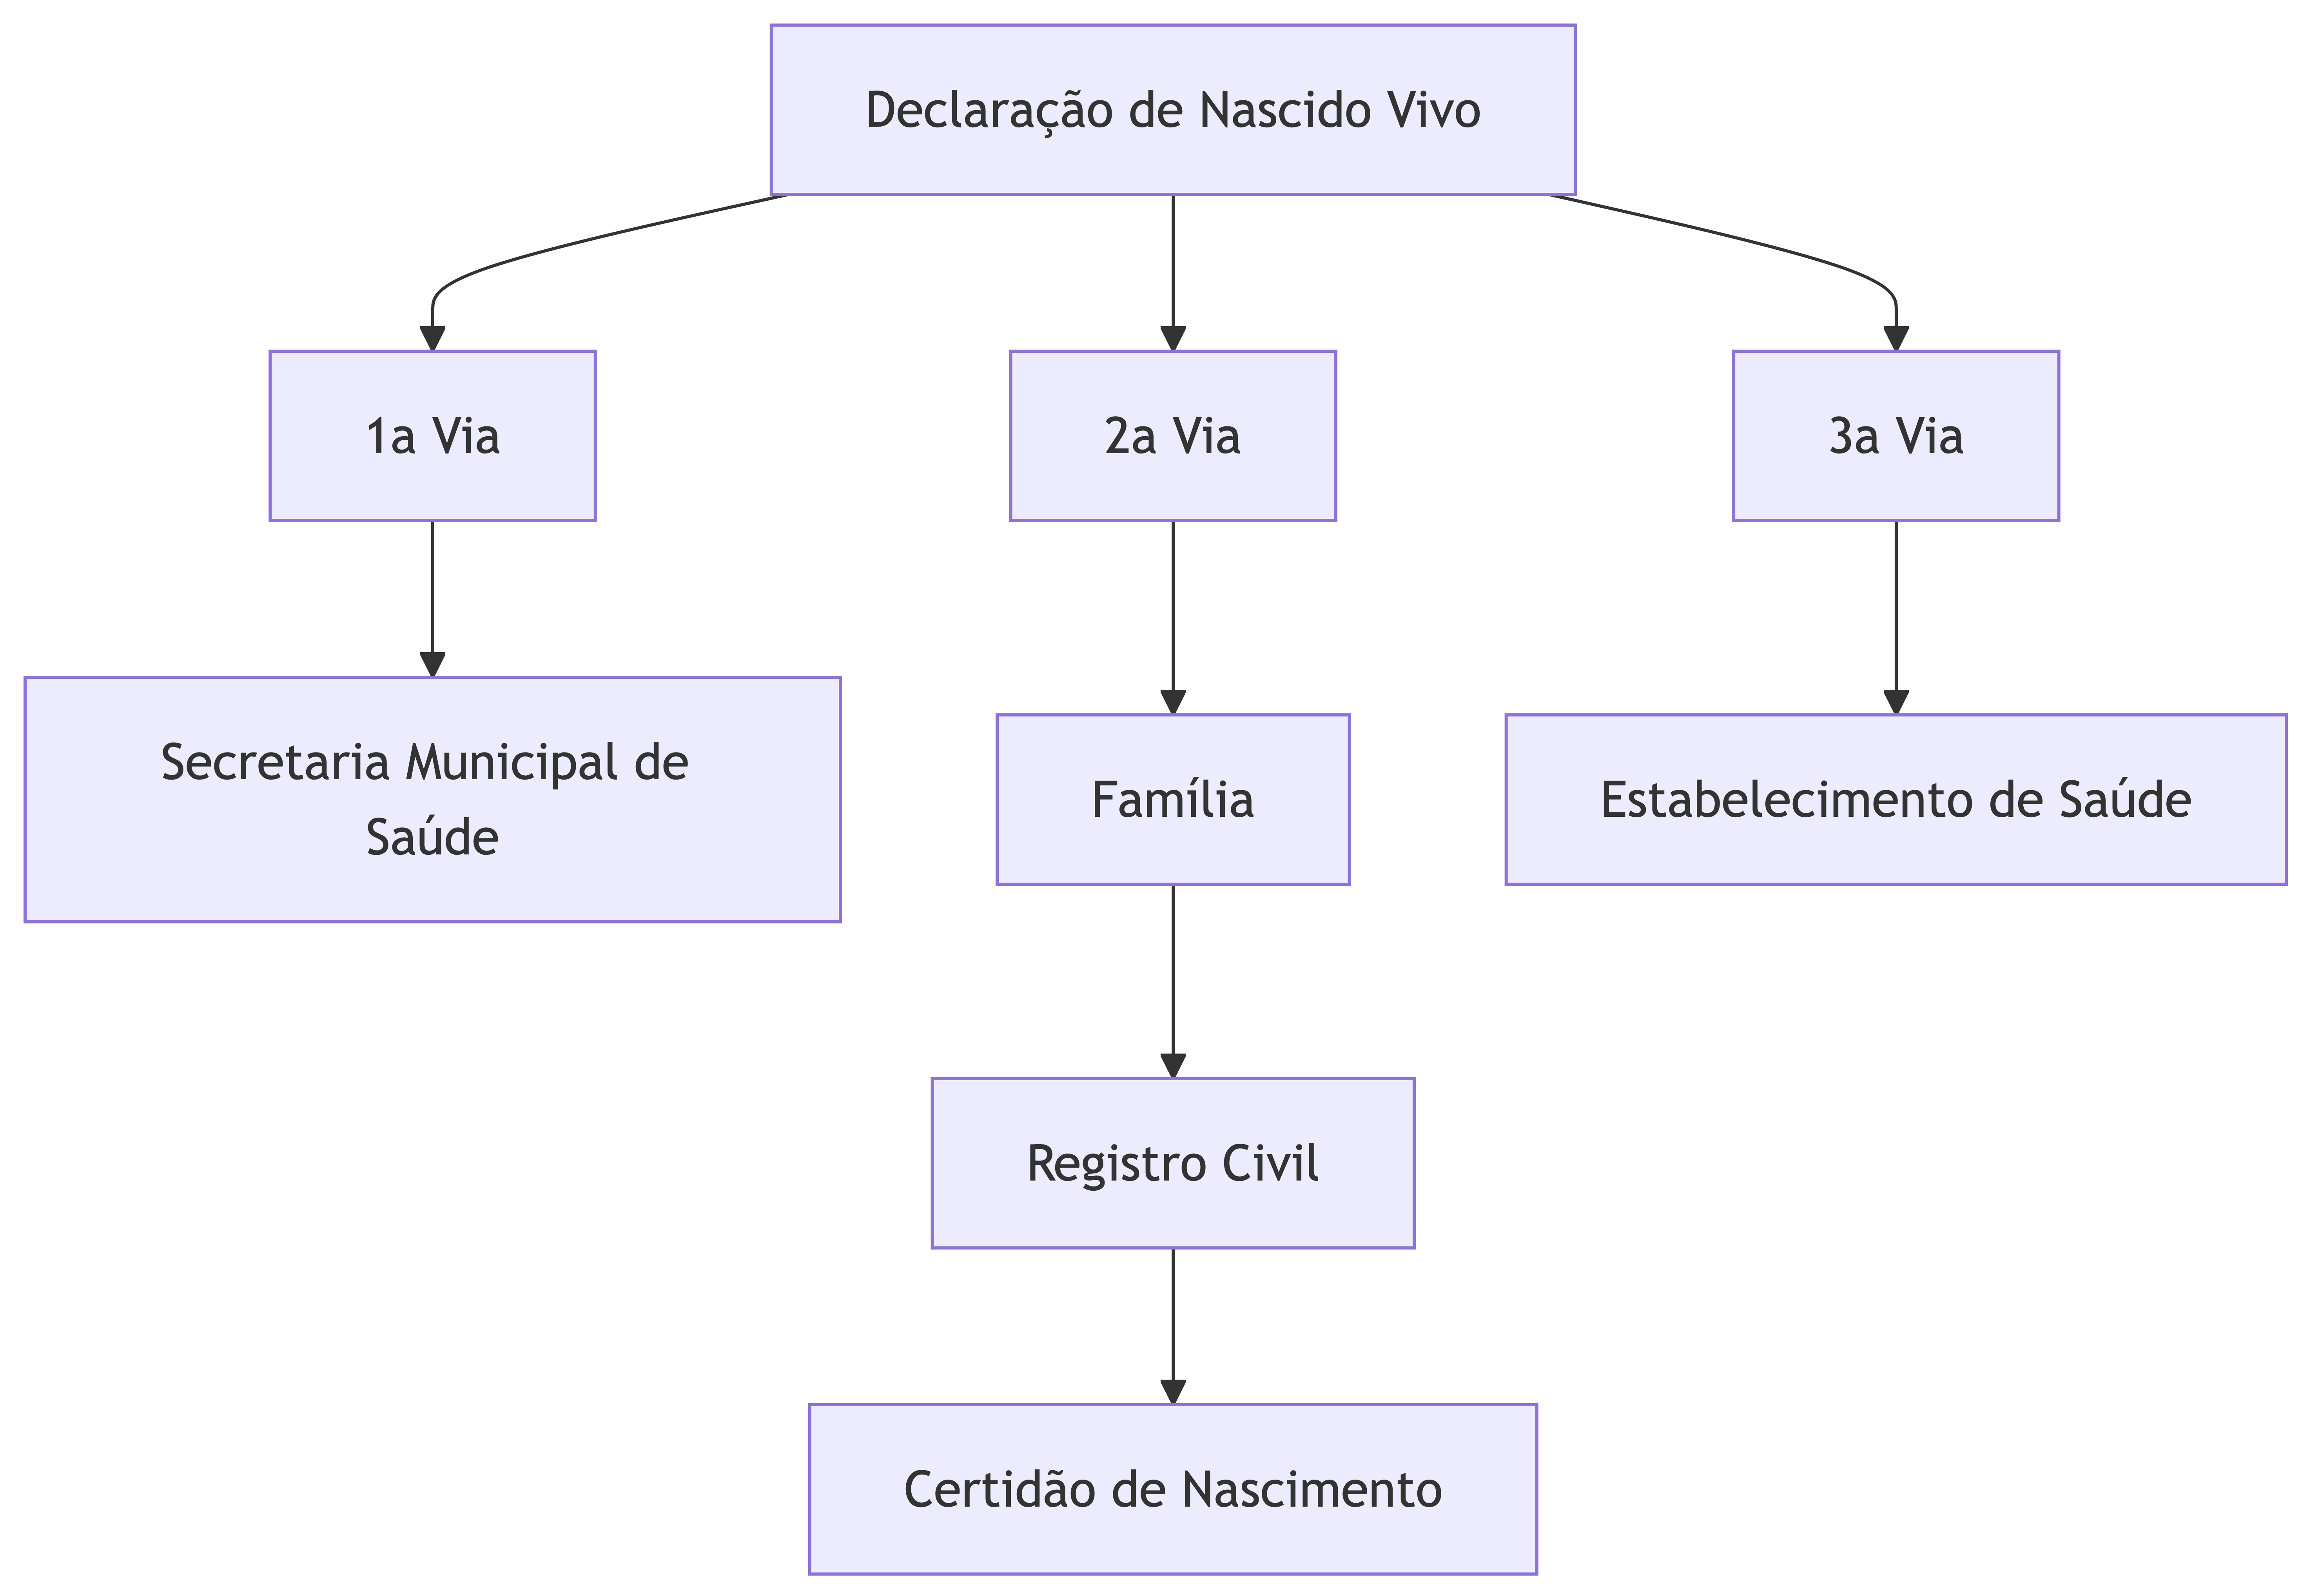
\includegraphics[width=11.76in,height=3.15in]{sim_files/figure-latex/mermaid-figure-1.png}

}

\caption{\label{fig-do}Fluxo de emissão e destinação das vias da
Declaração de Óbito}

\end{figure}%

A DO é emitida para todos os tipos de óbito, incluindo óbitos fetais,
sendo preenchida por um médico ou, quando da ausência de um médico, o
preenchimento é realizando em cartório, diante de testemunhas. Neste
documento consta a \emph{causa básica do óbito} e demais \emph{causas
secundárias}, que são codificadas conforme a Classificação Internacional
de Doenças (CID). Este dado é de grande importância para estudos em
saúde, possibilitando acompanhar as principais causas de óbitos em
diferentes grupos de doenças e recortes sociais.

A partir de 1979, o SIM passou a apresentar dados consolidados e, desde
então, a qualidade de seu preenchimento vem sendo aprimorada,
principalmente sobre os dados referentes a idade, raça/cor e existência
de gravidez. O maior desafio do SIM é a correta definição da causa
básica da morte, ainda sendo encontrado um número excessivo de
declarações de óbito com causas mal definidas (SENNA, 2009).

Mais informações sobre o preenchimento dos dados do SIM estão
disponíveis no
\href{assets/sim/declaracao-obito-manual-instrucoes-preenchimento.pdf}{manual
de preenchimento}, disponibilizado pelo Ministério da Saúde.

\section{Modelo da Declaração de
Óbito}\label{modelo-da-declarauxe7uxe3o-de-uxf3bito}

\begin{figure}

{\centering \pandocbounded{\includegraphics[keepaspectratio]{images/Wikipedia-Declaração_de_óbito_Brasil.jpg}}

}

\caption{Modelo de Declaração de Óbito}

\end{figure}%

\section{Estrutura e dicionário de
dados}\label{estrutura-e-dicionuxe1rio-de-dados}

Confira o documento de
\href{assets/sim/Estrutura_SIM_para_CD.pdf}{estrutura do SIM}.

\section{Acesso aos dados}\label{acesso-aos-dados}

\subsection{TabNet}\label{tabnet}

Os dados do SIM podem ser acessados no sistema TabNet do DataSUS, na
seção de Estatísticas Vitais.

\begin{itemize}
\tightlist
\item
  \href{https://datasus.saude.gov.br/mortalidade-desde-1996-pela-cid-10}{TabNet
  SIM}
\end{itemize}

\subsection{TabWin}\label{tabwin}

Para uso no TabWin, você irá precisar baixar no servidor de FTP do
DataSUS, os arquivos de dados no formato DBC e os arquivos auxiliares
para tabulação.

\begin{itemize}
\tightlist
\item
  \href{https://datasus.saude.gov.br/transferencia-de-arquivos/}{TabWin
  - Transferência de arquivos}
\end{itemize}

\subsection{R}\label{r}

Você pode usar o pacote
\href{https://rfsaldanha.github.io/microdatasus/index.html}{\texttt{\{microdatasus\}}}.

\begin{Shaded}
\begin{Highlighting}[]
\FunctionTok{library}\NormalTok{(microdatasus)}

\NormalTok{sim\_raw }\OtherTok{\textless{}{-}} \FunctionTok{fetch\_datasus}\NormalTok{(}
  \AttributeTok{year\_start =} \DecValTok{2021}\NormalTok{,}
  \AttributeTok{year\_end =} \DecValTok{2021}\NormalTok{,}
  \AttributeTok{uf =} \StringTok{"AC"}\NormalTok{,}
  \AttributeTok{information\_system =} \StringTok{"SIM{-}DO"}
\NormalTok{)}

\NormalTok{sim\_p }\OtherTok{\textless{}{-}} \FunctionTok{process\_sim}\NormalTok{(sim\_raw)}

\NormalTok{sim\_p}
\end{Highlighting}
\end{Shaded}

\begin{verbatim}
# A tibble: 5,496 x 111
   ORIGEM TIPOBITO  DTOBITO    HORAOBITO CODMUNNATU DTNASC   IDADE SEXO  RACACOR
   <chr>  <chr>     <chr>      <chr>     <chr>      <chr>    <chr> <chr> <chr>  
 1 1      Não Fetal 2021-03-23 1500      110020     1962-06~ 458   Masc~ Parda  
 2 1      Não Fetal 2021-03-23 0243      120050     1971-02~ 450   Masc~ Parda  
 3 1      Não Fetal 2021-03-23 1310      120040     1956-10~ 464   Femi~ Parda  
 4 1      Não Fetal 2021-04-17 2149      120050     1999-01~ 422   Masc~ Parda  
 5 1      Não Fetal 2021-01-06 0420      120020     2020-08~ 304   Masc~ Parda  
 6 1      Não Fetal 2021-02-06 1145      120034     1943-12~ 477   Masc~ Parda  
 7 1      Não Fetal 2021-02-15 <NA>      120050     1970-06~ 450   Masc~ Parda  
 8 1      Não Fetal 2021-02-16 0720      120060     1935-01~ 486   Masc~ Preta  
 9 1      Não Fetal 2021-02-15 1320      120050     1951-04~ 469   Femi~ Amarela
10 1      Não Fetal 2021-02-13 0700      120050     1957-02~ 464   Masc~ Parda  
# i 5,486 more rows
# i 102 more variables: ESTCIV <chr>, ESC <chr>, ESC2010 <chr>,
#   SERIESCFAL <chr>, CODMUNRES <chr>, LOCOCOR <chr>, CODESTAB <chr>,
#   ESTABDESCR <chr>, CODMUNOCOR <chr>, IDADEMAE <chr>, ESCMAE <chr>,
#   ESCMAE2010 <chr>, SERIESCMAE <chr>, QTDFILVIVO <chr>, QTDFILMORT <chr>,
#   GRAVIDEZ <chr>, SEMAGESTAC <chr>, GESTACAO <chr>, PARTO <chr>,
#   OBITOPARTO <chr>, PESO <chr>, TPMORTEOCO <chr>, OBITOGRAV <chr>, ...
\end{verbatim}

\subsection{PCDaS}\label{pcdas}

Os dados do SIM estão disponíveis na PCDaS para acesso via
\emph{notebooks}.

\begin{itemize}
\tightlist
\item
  \href{https://pcdas.icict.fiocruz.br/conjunto-de-dados/sistema-de-informacoes-de-mortalidade-sim/}{Dados
  SIM}
\item
  \href{https://pcdas.icict.fiocruz.br/conjunto-de-dados/sistema-de-informacao-sobre-mortalidade-declaracao-de-obitos-fetais-sim-dofet/}{Dados
  SIM-DOFET}
\end{itemize}

\subsection{Outras formas}\label{outras-formas}

Dados em formato CSV estão sendo disponibilizados no site OpenDataSUS,
mantido pelo DataSUS, incluindo versões de dados preliminares do ano
corrente.

\begin{itemize}
\tightlist
\item
  \href{https://opendatasus.saude.gov.br/dataset/sim}{OpenDataSUS - SIM}
\end{itemize}

\section{Principais usos e
indicadores}\label{principais-usos-e-indicadores}

Segundo a RIPSA (INFORMAÇÃO PARA A SAÚDE, 2008), os dados do SIM são
utilizados na construção de diversos indicadores de mortalidade. Pode-se
destacar os seguintes:

\begin{itemize}
\tightlist
\item
  Taxa de mortalidade infantil
\item
  Taxas de mortalidade neonatal precoce e tardia, pós-neonatal e
  perinatal
\item
  Taxa de mortalidade em menores de cinco anos
\item
  Razão de mortalidade materna
\item
  Mortalidade proporcional por grupos de causas
\end{itemize}

\section{Bibliografia recomendada}\label{bibliografia-recomendada}

\subsection{Documentos auxiliares}\label{documentos-auxiliares}

\begin{itemize}
\tightlist
\item
  \href{assets/sim/INTRO.pdf}{Histórico do SIM}
\item
  \href{assets/sim/Estrutura_SIM_para_CD.pdf}{Estrutura do SIM}
\item
  \href{assets/sim/declaracao-obito-manual-instrucoes-preenchimento.pdf}{Manual
  de preenchimento da Declaração de Óbito}
\item
  \href{assets/sim/a-declaracao-de-obito-documento-necessario-e-importante.pdf}{A
  Declaração de Óbito: documento necessário e importante}
\end{itemize}

\subsection{Vídeos recomendados}\label{vuxeddeos-recomendados}

\url{https://www.youtube.com/watch?v=I_wFPYkDbF8}

\url{https://www.youtube.com/watch?v=DuyB5bsz7yM}

\subsection{Qualidade do preenchimento dos
dados}\label{qualidade-do-preenchimento-dos-dados}

\subsection{Indicadores de saúde}\label{indicadores-de-sauxfade}

\bookmarksetup{startatroot}

\chapter{SINASC -- Sistema de Informação sobre Nascidos
Vivos}\label{sinasc-sistema-de-informauxe7uxe3o-sobre-nascidos-vivos}

\bookmarksetup{startatroot}

\chapter{SIH -- Sistema de Informações
Hospitalares}\label{sih-sistema-de-informauxe7uxf5es-hospitalares}

\bookmarksetup{startatroot}

\chapter{SIA -- Sistema de Informações
Ambulatoriais}\label{sia-sistema-de-informauxe7uxf5es-ambulatoriais}

\bookmarksetup{startatroot}

\chapter{CNES -- Cadastro Nacional de Estabelecimentos de
Saúde}\label{cnes-cadastro-nacional-de-estabelecimentos-de-sauxfade}

\bookmarksetup{startatroot}

\chapter{SIAB -- Sistema de Informação de Atenção
Básica}\label{siab-sistema-de-informauxe7uxe3o-de-atenuxe7uxe3o-buxe1sica}

\bookmarksetup{startatroot}

\chapter{SINAN -- Sistema de Informação de Agravos de
Notificação}\label{sinan-sistema-de-informauxe7uxe3o-de-agravos-de-notificauxe7uxe3o}

\bookmarksetup{startatroot}

\chapter{SIVEP -- Sistema de Vigilância
Epidemiológica}\label{sivep-sistema-de-vigiluxe2ncia-epidemioluxf3gica}

\bookmarksetup{startatroot}

\chapter{SIOPS -- Sistema de Informações sobre Orçamentos Públicos em
Saúde}\label{siops-sistema-de-informauxe7uxf5es-sobre-oruxe7amentos-puxfablicos-em-sauxfade}

\bookmarksetup{startatroot}

\chapter{SIPNI -- Sistema de Informações do Programa Nacional de
Vacinação}\label{sipni-sistema-de-informauxe7uxf5es-do-programa-nacional-de-vacinauxe7uxe3o}

\bookmarksetup{startatroot}

\chapter*{Referências}\label{referuxeancias}
\addcontentsline{toc}{chapter}{Referências}

\markboth{Referências}{Referências}

\phantomsection\label{refs}
\begin{CSLReferences}{0}{1}
\bibitem[\citeproctext]{ref-abouzahrHealthInformationSystems2005}
ABOUZAHR, C.; BOERMA, T. Health Information Systems: The Foundations of
Public Health. \textbf{Bulletin of the World Health Organization}, 2005.

\bibitem[\citeproctext]{ref-brasilLei60151973}
BRASIL. Lei nº 6.015, de 31 de dezembro de 1973. \textbf{Presidência da
República}, 1973.

\bibitem[\citeproctext]{ref-brasilLei81421990}
BRASIL. Lei nº 8.142, de 28 de dezembro de 1990. \textbf{Presidência da
República}, b1990.

\bibitem[\citeproctext]{ref-brasilLei80801990}
BRASIL. Lei nº 8.080, de 19 de setembro de 1990. \textbf{Presidência da
República}, a1990.

\bibitem[\citeproctext]{ref-brasilDecreto1001991}
BRASIL. Decreto nº 100, de 16 de abril de 1991. \textbf{Presidência da
República}, 1991.

\bibitem[\citeproctext]{ref-brasilDecreto41942002}
BRASIL. Decreto nº 4.194, de 11 de abril de 2002. \textbf{Presidência da
República}, a2002.

\bibitem[\citeproctext]{ref-ministeriodasaudeRelatorioFinal5a1975}
BRASIL, M. DA S. \textbf{Relat{ó}rio {Final} Da 5a {Confer{ê}ncia
Nacional} de {Sa{ú}de}}. Bras{í}lia: MS, 1975.

\bibitem[\citeproctext]{ref-BrasilDataSUS2002}
BRASIL, M. DA S. \textbf{{DATASUS} {Trajet{ó}ria} 1991-2002}.
Bras{í}lia: Minist{é}rio da Sa{ú}de, 2002b.

\bibitem[\citeproctext]{ref-OPAS2008}
INFORMAÇÃO PARA A SAÚDE, R. I. DE. \textbf{Indicadores B{á}sicos Para a
Sa{ú}de No {Brasil}: Conceitos e Aplica{ç}{õ}es}. Bras{í}lia:
Organiza{ç}{ã}o Pan-Americana da Sa{ú}de, 2008.

\bibitem[\citeproctext]{ref-lippeveldRoutineHealthInformation2001}
LIPPEVELD, T. \textbf{Routine Health Information Systems: The Glue of a
Unified Health System}. Keynotes Address. \textbf{Anais}...Washington:
Workshop on Issues; Innovation in Routine Health Information in
Developing Countries, 2001.

\bibitem[\citeproctext]{ref-makrakisRegistroCivilNo2000}
MAKRAKIS, S. \textbf{{O Registro Civil no Brasil}}.
\{Disserta\{\textbackslash c c\}\{\textbackslash\textasciitilde a\}o de
Mestrado\}---Rio de Janeiro: Funda{ç}{ã}o Get{ú}lio Vargas, Escola
Brasileira de Administra{ç}{ã}o P{ú}blica, 2000.

\bibitem[\citeproctext]{ref-ministeriodasaudeExperienciaBrasileiraEm2009}
MINISTÉRIO DA SAÚDE, F. O. C., Organização Pan-Americana da Saúde.
\textbf{{A experi{ê}ncia brasileira em sistemas de informa{ç}{ã}o em
sa{ú}de}}. Bras{í}lia: Ministério da Saúde, 2009. v. 2

\bibitem[\citeproctext]{ref-sennaSistemaInformacoesSobre2009}
SENNA, M. DE C. M. Sistema de {Informa{ç}{õ}es} Sobre {Mortalidade}
({SIM}). Em: \textbf{A Experi{ê}ncia Brasileira Em Sistemas de
Informa{ç}{ã}o Em Sa{ú}de}. B. {Textos B{á}sicos} de {Sa{ú}de}.
Bras{í}lia: Minist{é}rio da Sa{ú}de, 2009. v. 2.

\bibitem[\citeproctext]{ref-viacavaSistemaInformacaoSobre2009}
VIACAVA, F. Sistema de {Informa{ç}{ã}o} Sobre {Nascidos Vivos}
({Sinasc}). Em: \textbf{A Experi{ê}ncia Brasileira Em Sistemas de
Informa{ç}{ã}o Em Sa{ú}de}. B. {Textos B{á}sicos} de {Sa{ú}de}.
Bras{í}lia: Minist{é}rio da Sa{ú}de, 2009. v. 2.

\bibitem[\citeproctext]{ref-worldhealthorganisationFrameworkStandardsCountry2008}
WHO. \textbf{Framework and Standards for Country Health Information
Systems}. 2. ed. Genebra: {[}s.n.{]}.

\end{CSLReferences}

\cleardoublepage
\phantomsection
\addcontentsline{toc}{part}{Apêndices}
\appendix

\chapter{CID -- Classificação Internacional de
Doenças}\label{cid-classificauxe7uxe3o-internacional-de-doenuxe7as}

\section{Histórico}\label{histuxf3rico}

\section{Estrutura}\label{estrutura}

\section{Edições da CID no Brasil}\label{ediuxe7uxf5es-da-cid-no-brasil}

\subsection{CID-9}\label{cid-9}

\subsection{CID-10}\label{cid-10}

\subsection{CID-11}\label{cid-11}

\chapter{Estimativas populacionais}\label{estimativas-populacionais}

\chapter{RNDS -- Rede Nacional de Dados em
Saúde}\label{rnds-rede-nacional-de-dados-em-sauxfade}




\end{document}
